\section{Datenbank}

\subsection{Allgemeines}

Um bei grösseren Datenmengen Speicherplatz zu sparen soll bei der grössten Tabelle (Items) weitgehend Integer als Feldtyp verwendet werden. In diesen ID Feldern soll die ID der Informationen aus den entsprechenden Untertabellen gespeichert werden, damit diese später in der App für den User angezeigt werden können und dieser nicht nur eine nicht aussagekräftige Zahl angezeigt bekommt.\\

Da SQLITE den Datentyp Boolean nicht kennt soll auch hier auf Integer zurück gegriffen werden. Alle solch verwendeten Felder werden nur mit 1 (true) und 0 (false) gefüllt.\\

Da auch der Datentyp Date in SQLITE nicht existiert soll hier auf String zurück gegriffen werden. Das Jahr wird hierbei als 4-stelliger String gespeichert. 

\subsection{Aufbau der SQLITE Datenbank}

Die Datenbank der App hat folgende Tabellen und Felder.

\begin{longtable}{|l|l|l|l|}
	\rowcolor{black} {\color{white}\textbf{}} & {\color{white}\textbf{Typ}} & {\color{white}\textbf{Key}} & {\color{white}\textbf{Information/Verwendung}} \\
	\textbf{Items} & & & Table in welchem alle Informationen eines Items gespeichert werden. \\ \hline
	\rowcolor{DarkSeaGreen} ITEM\_ID & Integer & Ja & Id des Items. \\ \hline
	EAN & Integer & & Barcode des Items. \\ \hline
	\rowcolor{DarkSeaGreen} TITLE & String & & Name des Items. \\ \hline	
	RATING & Integer & & Von 0 bis 5 Sterne das persönliche Rating des Users. \\ \hline
	\rowcolor{DarkSeaGreen} MEDIA\_TYPE & String & & Art des Items: Book, Movie oder Game. \\ \hline
	GENRE\_ID & Integer &  & ID des Genres kann für alle Arten von Items verwendet werden. \\ \hline
	\rowcolor{DarkSeaGreen} LANGUAGE\_ID & Integer & & ID der Sprache des Items. \\ \hline
	LAUNCH & String & & Erscheinungsjahr des Items. \\ \hline
	\rowcolor{DarkSeaGreen} RENTAL & Integer & & Boolean (1 oder 0) welcher den Leihstatus angibt. \\ \hline
	PUBLISHER\_ID & Integer & & ID des Verlegers (nur Bücher). \\ \hline
	\rowcolor{DarkSeaGreen} AUTHOR\_ID & Integer & & ID des Autors (nur Bücher). \\ \hline
	SYSTEM\_ID & Integer & & ID des Systems (nur Spiele) \\ \hline
	\rowcolor{DarkSeaGreen} DVD & Integer & & Boolean welcher angibt ob es sich um eine DVD handelt. \\ \hline
	BLURAY & Integer & & Boolean welcher angibt ob es sich um eine BluRay handelt. \\ \hline
	\rowcolor{DarkSeaGreen} STUDIO\_ID & Integer & & Id des Studio (Film und Spiel). \\ \hline
	DIRECTOR\_ID & Integer & & Id des Regisseur (nur Film). \\ \hline
	\rowcolor{DarkSeaGreen} PARENTAL & Integer & & Altersfreigabe des Items (Film und Spiel). \\ \hline
	REMARKS & String & & Bemerkungen des Users. \\ \hline
	\rowcolor{DarkSeaGreen} \textbf{History} & & & Tabelle mit der Verleih Historie. \\ \hline
	HISTORY\_ID & Integer & Ja & ID des Verleih Vorgangs. \\ \hline
	\rowcolor{DarkSeaGreen} ITEM\_ID & Integer & & ID des verliehenen Items. \\ \hline
	FRIEND\_ID & Integer & & ID des Freundes welcher das Item geliehen hat. \\ \hline
	\rowcolor{DarkSeaGreen} START & String & & Datum an welchen das Item verliehen wurde. \\ \hline
	BACK & String & & Datum an welchem das Item wieder zurück gegeben wurde. \\ \hline
	\rowcolor{DarkSeaGreen} \textbf{Friends} & & & Tabelle in welchem alle Freunde hinterlegt sind. \\ \hline
	FRIEND\_ID & Integer & Ja & ID des Freundes. \\ \hline
	\rowcolor{DarkSeaGreen} FIRST\_NAME & String & & Vorname des Freundes. \\ \hline
	LAST\_NAME & String & & Nachname des Freundes. \\ \hline
	\rowcolor{DarkSeaGreen} \textbf{Authors} & & & Tabelle mit allen Autoren.  \\ \hline
	AUTHOR\_ID & Integer & Ja & ID des Autors. \\ \hline
	\rowcolor{DarkSeaGreen} AUTHOR & String & & Name des Autors. \\ \hline
	\textbf{Directors} & & & Tabelle mit allen Regisseuren. \\ \hline
	\rowcolor{DarkSeaGreen} DIRECTOR\_ID & Integer & Ja & ID des Regisseur. \\ \hline
	DIRECTOR & String & & Name des Regisseur. \\ \hline
	\rowcolor{DarkSeaGreen} \textbf{Genres} & & & Tabelle mit allen Genres. \\ \hline
	GENRE\_ID & Integer & Ja & ID des Genres. \\ \hline
	\rowcolor{DarkSeaGreen} GENRE & String & & Genre \\ \hline
	\textbf{Languages} & & & Tabelle welche alle Sprachen enthält. \\ \hline
	\rowcolor{DarkSeaGreen} LANGUAGE\_ID & Integer & Ja & ID der Sprache \\ \hline
	LANGUAGE & String & & Sprache \\ \hline
	\rowcolor{DarkSeaGreen} \textbf{Publishers} & & & Tabelle welche alle Verlage enthält. \\ \hline
	PUBLISHER\_ID & Integer & Ja & ID des Verlags. \\ \hline
	\rowcolor{DarkSeaGreen} PUBLISHER & String & & Name des Verlags. \\ \hline
	\textbf{Studios} & & & Welche alle Studios enthält. \\ \hline
	\rowcolor{DarkSeaGreen} STUDIO\_ID & Integer & Ja & ID des Studios. \\ \hline
	STUDIO & String & & Name des Studios. \\ \hline
	\rowcolor{DarkSeaGreen} \textbf{Systems} & & & Tabelle welche alle Systeme enthält. \\ \hline
	SYSTEM\_ID & Integer & Ja & ID des Systems. \\ \hline
	\rowcolor{DarkSeaGreen} SYSTEM & String & & Name des Systems. \\ \hline
\end{longtable}

\newpage

\begin{landscape}
	\subsection{Übersicht Datenbank}
	\label{subsec:UebersichtDB}
	\begin{figure}[htbp]
		\centering
		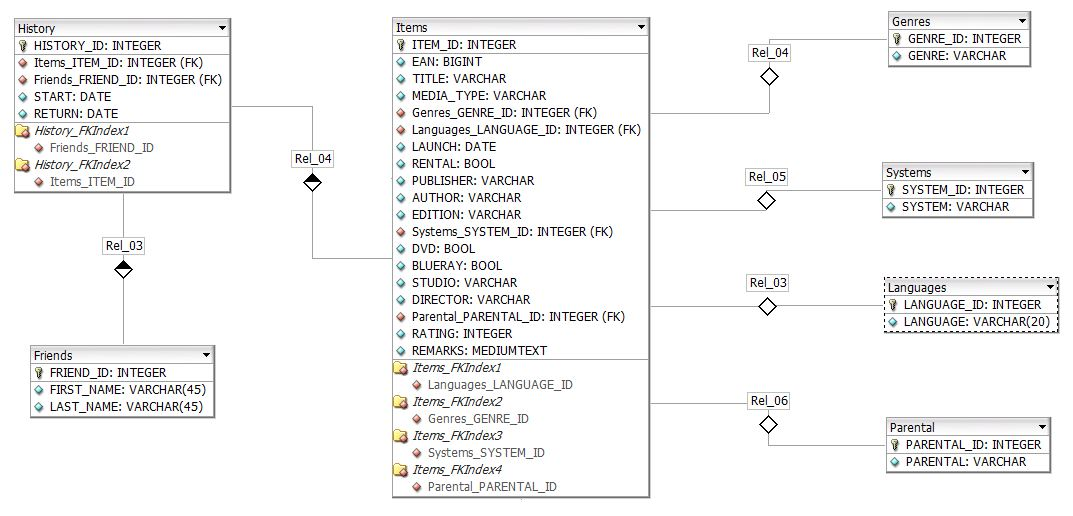
\includegraphics[scale=0.6]{pic/DbDesign}
		\caption{Überblick Datenbank}
	\end{figure}
\end{landscape}